\begin{center}
\section{Design}
\label{design}
\end{center}

Breaking the problem down into building blocks of abstract classes and interfaces allows each system to define how it should interact and behave. As mentioned in Section\ref{sec:API}, creational patterns are valuable techniques for constructing large-scale systems. Combining Builder classes and API is the basis for how the system is structured.

\begin{figure}[H]
    \centering
    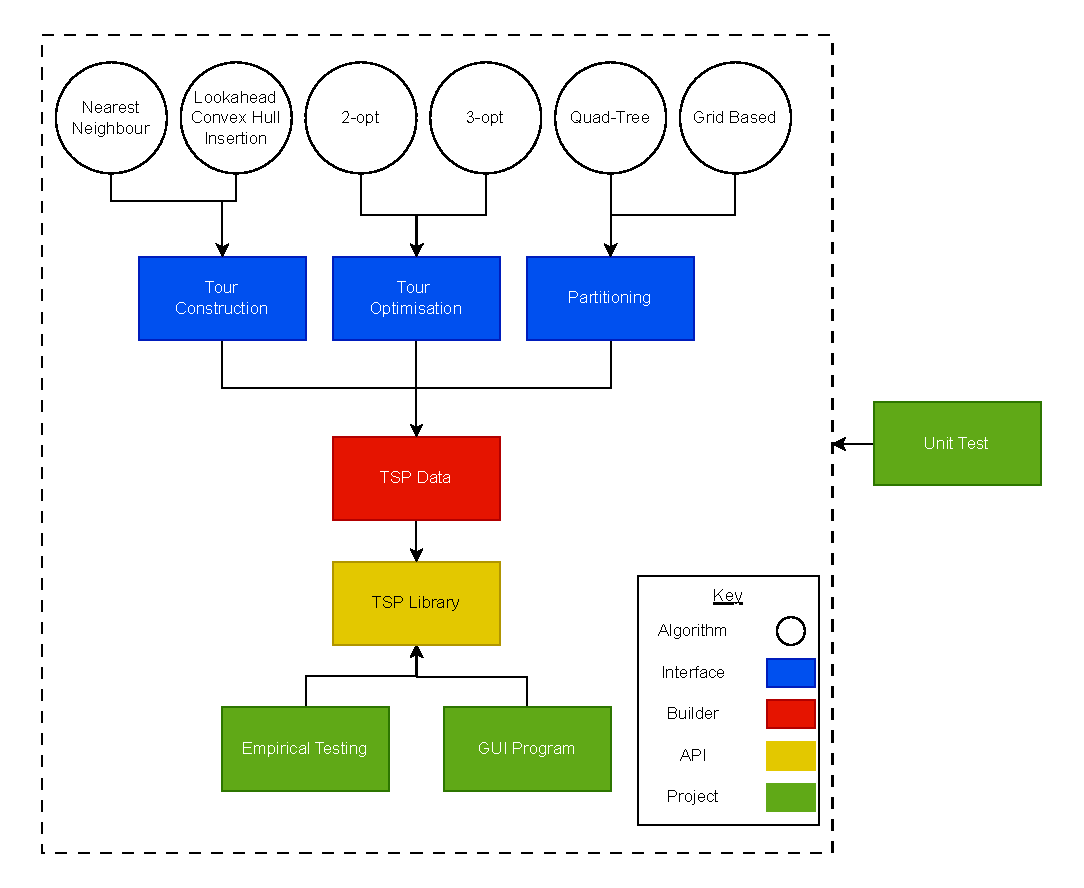
\includegraphics[width=1\textwidth]{sections/image/Class_Diagram-Basic.drawio.pdf}
    \caption{Class Structure}
    \label{fig:classdia}
\end{figure}

Figure\ref{fig:classdia} illustrates the class hierarchy and the interactions between each system block for the core static library code. At each level, a layer of abstraction is applied to hide information about the other blocks, allowing them to work independently.

\subsection{TSP Library API}
\begin{figure}[H]
    \centering
    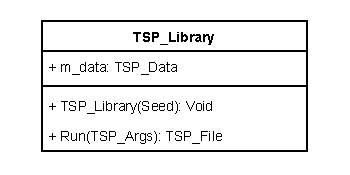
\includegraphics[width=0.6\textwidth]{sections/image/Class_Diagram-TSP_Lib.drawio.pdf}
    \caption{TSP Lib}
    \label{fig:TSP_Lib}
\end{figure}

The TSP Library serves as the entry point for the static library, providing the API that controls the creation and execution of TSP algorithms through the TSP\_data class. It is responsible for parsing the data and serialising the result. It houses all the asynchronous timeout code and benchmarking functionality.

There are only two functions: the constructor and the run function. The constructor uses a seed value to generate m\_data as a composition object with all the data required for the functionality. The run function controls the handling of timeouts, the execution of the algorithm steps, and data serialisation to the TSP\_File type. The ordering of the run function is as follows:

\begin{enumerate}
    \item Start benchmark timer
    \item Initialise partitioning data
    \item Initialise caching data
    \item Run tour constructor algorithm
    \item Run tour optimiser algorithm
    \item Stop benchmark timer
    \item Validate the route
    \item Process data and serialise to TSP\_File
\end{enumerate}

\subsubsection{TSP File}
\label{sec:TSP_File}
\begin{figure}[H]
    \centering
    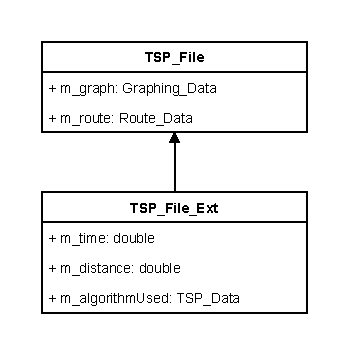
\includegraphics[width=0.5\textwidth]{sections/image/Class_Diagram-TSP_File.drawio.pdf}
    \caption{TSP File}
    \label{fig:TSP_File}
\end{figure}

TSP\_File represents multiple classes for deserialising and serialising the `.TSP' file type, which originates from the TSPLib format. The original file type contains relevant information to reconstruct the problem and its solution. For this project, the file type was expanded using polymorphism by adding benchmarking statistics with the class TSP\_File\_Ext.

\subsection{TSP Data API}
\label{tspData}

\begin{figure}[H]
    \centering
    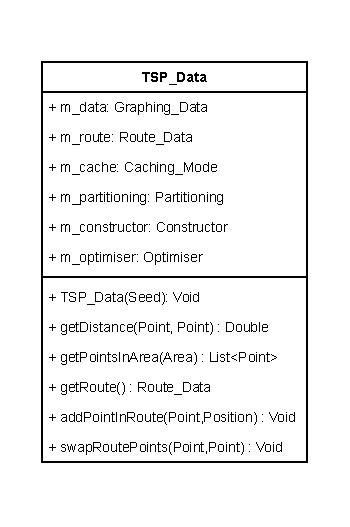
\includegraphics[width=0.5\textwidth]{sections/image/Class_Diagram-TSP_Data.drawio.pdf}
    \caption{TSP Data}
    \label{fig:TSP_Data}
\end{figure}

TSP\_Data is what connects everything together and ensures the TSP properties are kept. It is a builder class(Section\ref{sec:API}) for generating any variation of TSP algorithm from the number of TSP Modules(Section\ref{modules}). It stores the graph theory and route creation data and logic, serving as an API(Table\ref{tab:functions}) for the composition objects and forcing them to utilise the caching(getDistance) and partitioning(getPointsInArea) techniques. The class isolates the raw data from other classes to prevent data corruption and ensure the properties of the Travelling Salesman Problem(addPointInRoute \& swapRoutePoints) are maintained. The tour constructor uses the addPointInRoute() function, and tour optimisers uses swapRoutePoints(), as seen from Figure\ref{twosubprocedure}.

\begin{table}[H]
    \centering
    \renewcommand{\arraystretch}{1.2} % Adjust row height for readability
    \begin{tabularx}{\textwidth}{|p{3.2cm}|p{2.5cm}|p{2.5cm}|X|}
\hline
{\ul \textbf{Function}} & {\ul \textbf{Argument}} & {\ul \textbf{Return}} & {\ul \textbf{Description}}                                                       \\ \hline
TSP\_Data()             & Random Seed             & Void                  & Constructor: Generate a random problem                                           \\ \hline
getDistance()           & Point \& Point          & Double      & Checks the cache table or generates the Euclidean distance between two points         \\ \hline
getPointInArea()        & Area                    & List of Points        & Uses the partitioning algorithm to fetch all the points within a geographical area \\ \hline
getRoute()              & Null                    & List of Points        & Returns current route                                                            \\ \hline
addPointInRoute()       & Point \& Position       & Null                  & Adds point to the position in the route                                          \\ \hline
swapRoutePoints()       & Point \& Point          & Null                  & Swaps two points in the route                                                    \\ \hline
    \end{tabularx}
    \caption{Function Definition}
    \label{tab:functions}
\end{table}


\subsection{TSP Modules Interfaces}
\label{modules}

Interfaces or pure virtual classes in C++(Section\ref{sec:API}) dictate the interaction through which to communicate with a block. The interface acts as a conduit between TSP\_Data and the underlying algorithms and functionality(Figure\ref{fig:modules}). Because the modules only need to interact statically with TSP\_Data and they are situated in composition, a reference is all that is required for modules to access the API(Section\ref{tspData}).

\begin{figure}[H]
    \centering
    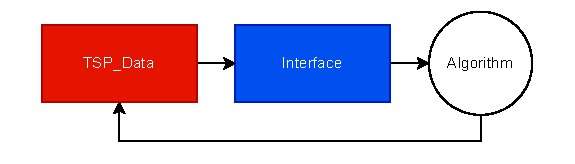
\includegraphics[width=0.7\textwidth]{sections/image/Class_Diagram-Page-5.drawio.pdf}
    \caption{Modules Interface Interaction}
    \label{fig:modules}
\end{figure}

The program employs this technique in four locations: the tour constructor, the tour optimiser, partitioning, and caching. For tour constructors and optimisers, the interface handles the uniform construction and destruction of every algorithm through a base process, runConstructor() and runOptimiser(). The partitioning interface requires the underlying partition type(Section\ref{partitioning}) to have both a construction method and a method for determining points within an area. Caching similarly requires a construction method and a distance between points. Interfaces are a requirement because each implementation utilises a distinct memory structure and logic to achieve the same functionality, as shown in Figure\ref{fig:part_example}.

\begin{figure}[H]
    \centering
        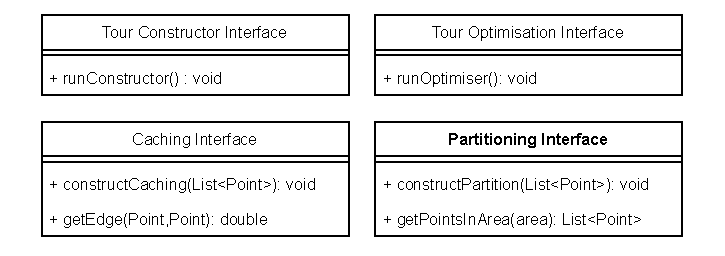
\includegraphics[width=\textwidth]{sections/image/Class_Diagram-Page-7.drawio.pdf}
        \caption{Interface Descriptions}
    \label{fig:}
\end{figure}

\begin{figure}[H]
    \centering
    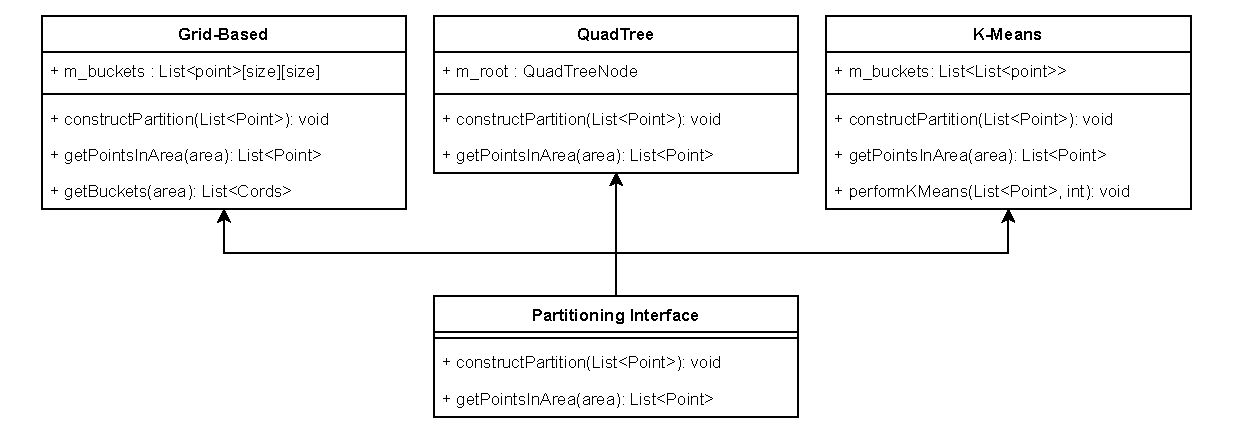
\includegraphics[width=\textwidth]{sections/image/Class_Diagram-Page-6.drawio.pdf}
    \caption{Partitioning Interface Example}
    \label{fig:part_example}
\end{figure}

\subsection{TSP Projects}

Projects are individual executables that compile shared and discrete code independently, each with its own set of compiler options and libraries. Mixing GUI applications and background applications presents numerous issues and increases complexity when the two applications are disjointed. Therefore, keeping each application's specific code and compiler options separate improves development time and user application efficiency. If the applications require shared code, that shared code should be placed in a static library(Section\ref{sec:c++}), which is what the TSP Library is. This report requires four projects: Empirical Testing Suite, GUI output, Unit test, and TSP File Reader.

\subsubsection{Empirical Testing Suite}
\label{sec:testing}
The Empirical Testing Suite is a Command-Line Interface(CLI) application for selecting and starting the process of testing various algorithms, serving as the primary component of the report and following the methodology listed in Section\ref{method}. It supports simultaneous testing and multiple test suite designs. It is responsible for creating, appending, and saving the result data to a file(More in Section\ref{filesystem}). There are multiple different test suites that serve different purposes:

\begin{table}[H]
    \centering
    \renewcommand{\arraystretch}{1.2} % Adjust row height for readability
    \begin{tabularx}{\textwidth}{|p{3cm}|X|X|}
    \hline
{\ul \textbf{Name}}           & {\ul \textbf{Function}}                                   & {\ul \textbf{Aim}}                                                             \\ \hline
Basic Test                    & Runs every algorithm for a given problem size             & Generates simple data for each algorithm                                             \\ \hline
Multi Test                    & Runs every algorithm for multiple different problem sizes & Generates a wide range of data for every algorithm                                   \\ \hline
Dynamic Test                  & Runs only SLACIH and DLACIH for a given problem size      & Generates data for the optimal depth of SLACIH and comparative performance of DLACIH \\ \hline
Dynamic Args Gradient Descent & Performs gradient descent on DLACIH arguments             & Hyper-optimise the DLACIH arguments values                                                \\ \hline
TSPLib Test                   & Runs DLACIH on every Euclidean TSP in TSPLib              & Benchmark DLACIH against exact solutions                                       \\ \hline
    \end{tabularx}
    \caption{Test Suites}
    \label{tab:testsuites}
\end{table}

\begin{figure}[H]
    \centering
    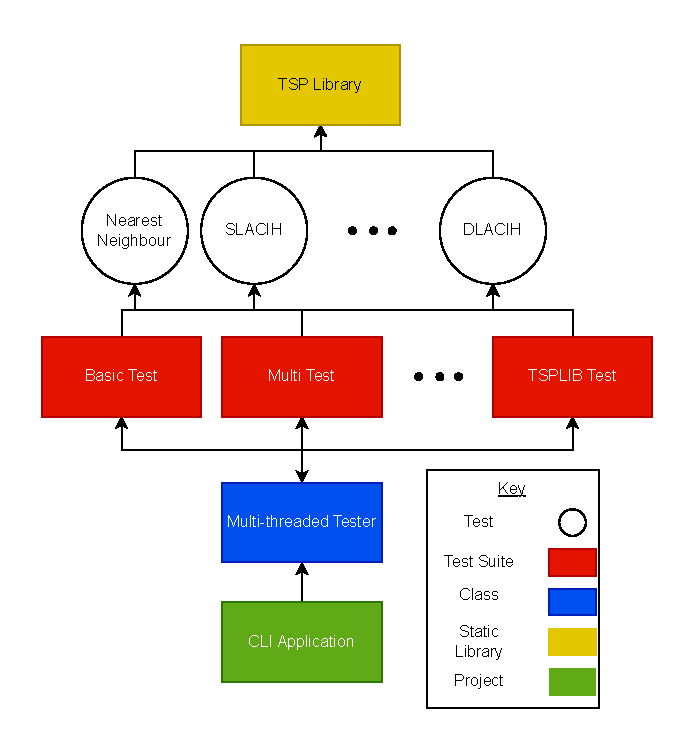
\includegraphics[width=0.75\textwidth]{sections/image/Class_Diagram-Page-8.drawio.pdf}
    \caption{Empirical Testing Suite Design}
    \label{fig:Emprical}
\end{figure}

The application block serves as the entry point, featuring only CLI menu logic and basic sanitation checks. It passes on the user inputs to the multi-threaded tester for execution. The menu collects inputs such as:
\begin{itemize}
    \item Which test suite to run
    \item How many iterations to run
    \item How long it should run for 
    \item What file type should it produce
\end{itemize}

The multi-threaded tester(Tester for short) is the core block, as it allows other classes to add tests to a queue for them to be run in parallel and adheres to the parameters set by the user. The Tester features an iterative, asynchronous loop that manages the continuous execution of the selected test suite and periodically writes the results to a file(Section\ref{filesystem} \& Figure\ref{fig:emp_scr}). The Tester limits the number of active tests to the number of cores available and executes a new test only once a thread from the active thread pool becomes available in a FIFO queue. Equipped in the terminal is a CTRL+C break command to gracefully stop the test mid-run, preventing file corruption.

\begin{figure}[H]
    \centering
    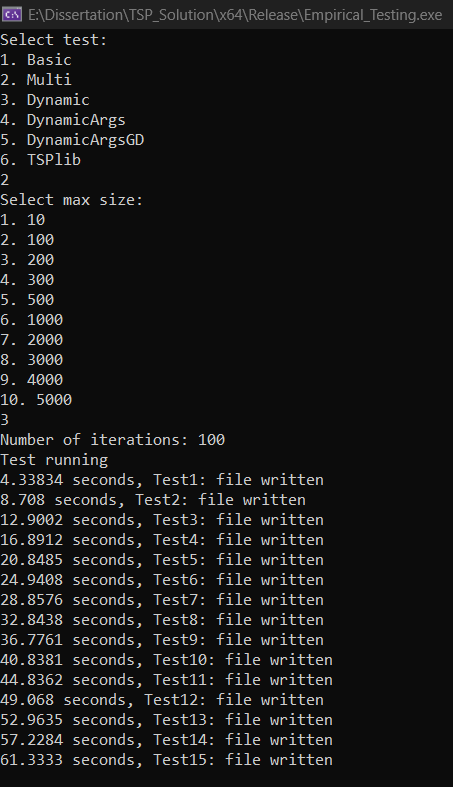
\includegraphics[width=0.35\textwidth]{sections/image/Screenshot 2025-04-08 111230.png}
    \caption{Empirical Test Suite}
    \label{fig:emp_scr}
\end{figure}

The test blocks(black circle in Figure\ref{fig:Emprical}) are individual tests that act as a wrapper(also known as an adaptor) for running an algorithm on the TSP Library with some given parameters. The test suite blocks(red rectangles in Figure\ref{fig:Emprical}) are predefined sets of tests that load the test blocks into the multi-threaded tester. Each test suite has a design it is trying to evaluate, and they do not behave equally. The test suite TSPLIB does not use random problems and instead solves the Euclidean TSP contained in TSPLIB from the smallest to the largest problem. The test suite Dynamic Args Gradient Descent(Table\ref{tab:testsuites}) uses the same five problems for each iteration of the gradient descent.

\subsubsection{TSP GUI}
\begin{figure}[H]
    \centering
    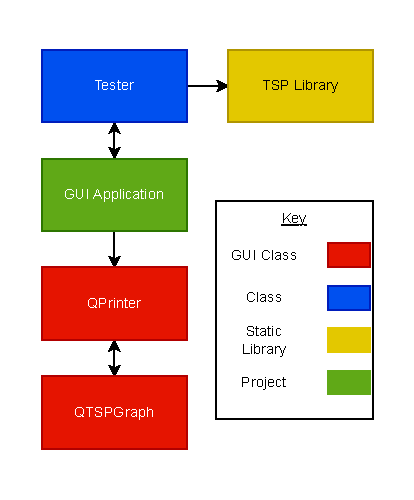
\includegraphics[width=0.5\textwidth]{sections/image/Class_Diagram-Page-9.drawio.pdf}
    \caption{TSP GUI Design}
    \label{fig:guidesign}
\end{figure}

Euclidean TSP belongs to the geometric space, therefore, the points and edges of the graph problem can be represented on a two-dimensional plane. This can be displayed on a GUI application to verify and analyse solutions. This is achieved through QT6 and a paint system for drawing diagrams(Figure\ref{fig:TSPGUI}). The GUI application runs in two steps: it runs algorithms on a TSP, then displays the solution. The two steps do not interact, apart from passing the backend output into the frontend(Figure\ref{fig:guidesign}).

\begin{figure}[H]
    \centering
    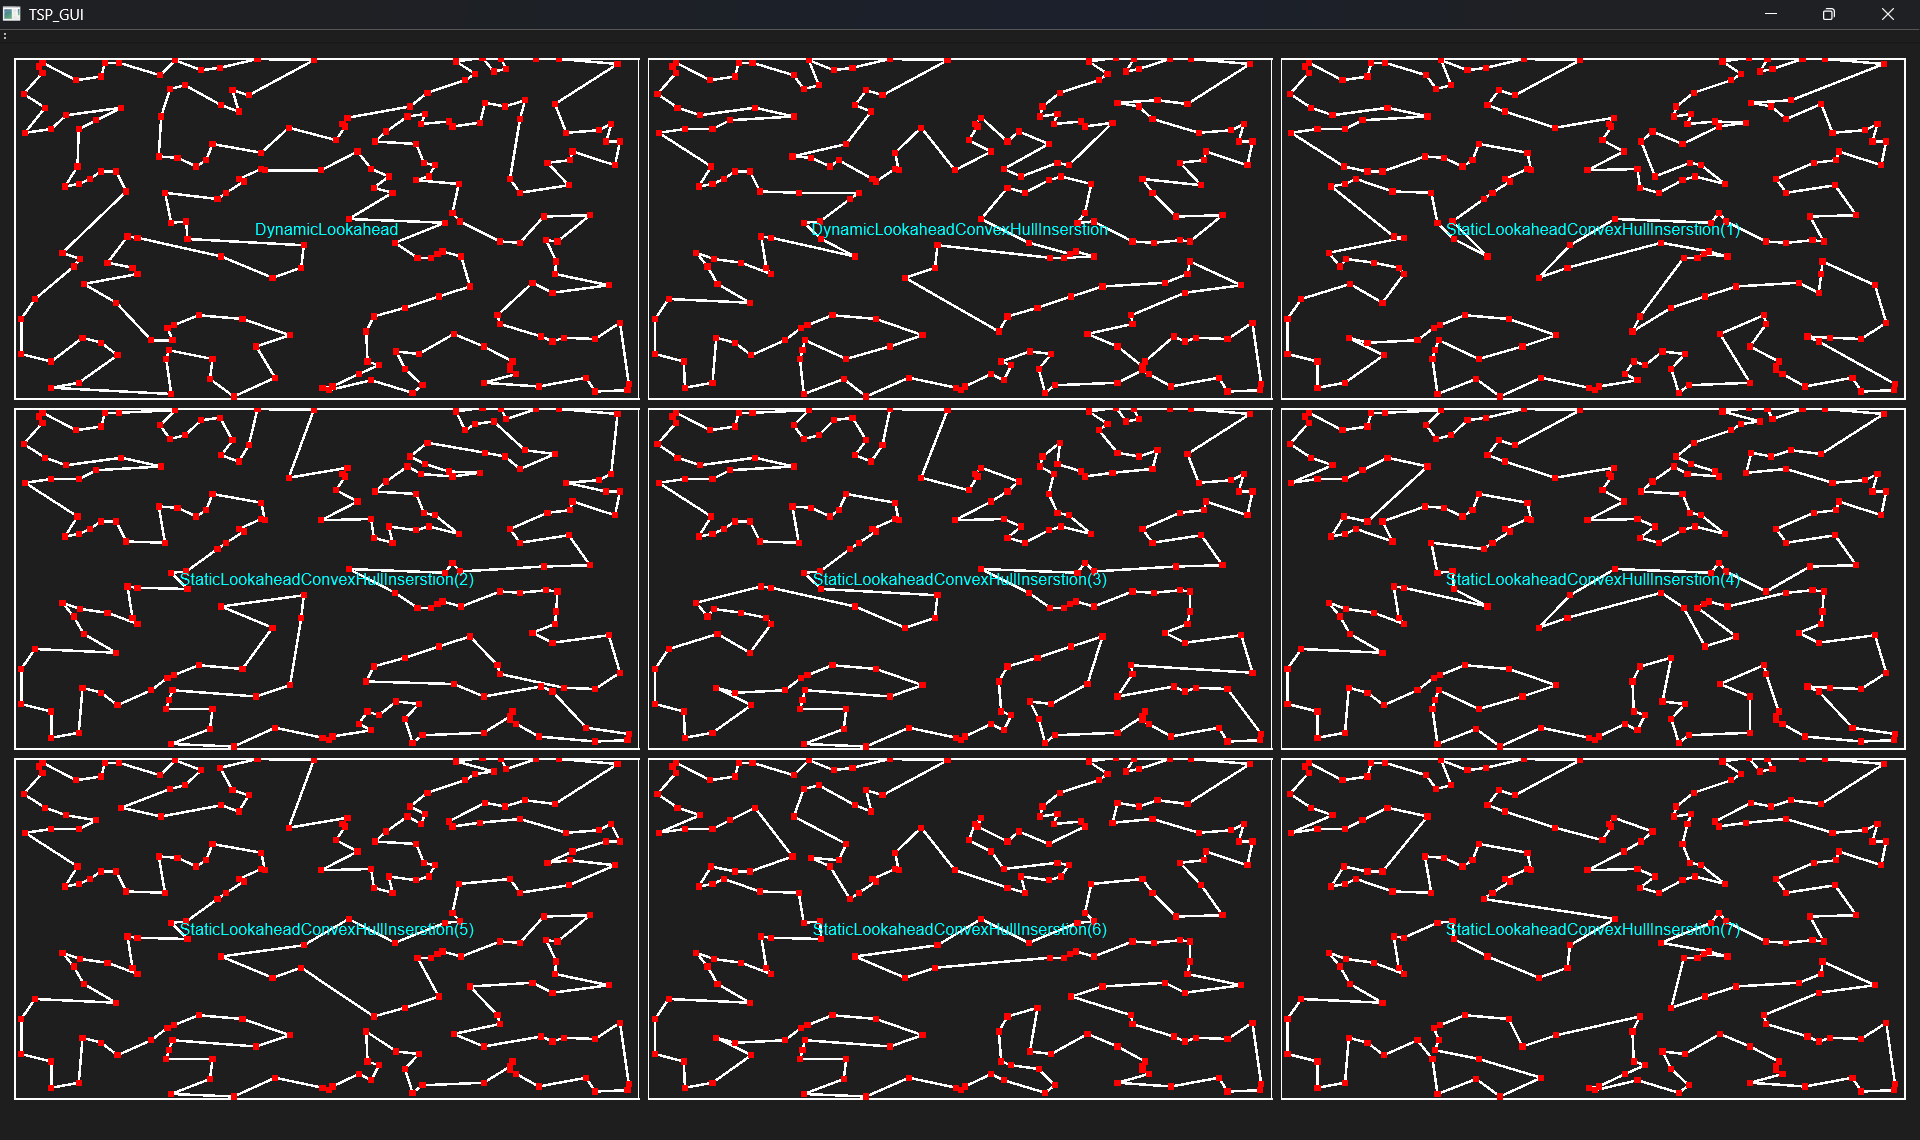
\includegraphics[width=0.95\textwidth]{sections/image/TSP_GUI.png}
    \caption{TSP GUI}
    \label{fig:TSPGUI}
\end{figure}



\subsubsection{Unit Test}
\label{designUnit}
C++ has a plethora of unit testing libraries, all with their pros and cons, but there are no wrong choices. GoogleTest\cite{googletest} is used for its simple integration into Visual Studio. In Figure\ref{fig:classdia}, the unit test encapsulates the entire code base as it can access and create any object needed for the test. This project followed the ``art of unit testing"\cite{osherove2013art} design for a good unit test, reducing complexity by testing only one variable and ensuring repeatable and predictable results.

\begin{figure}[H]
    \centering
    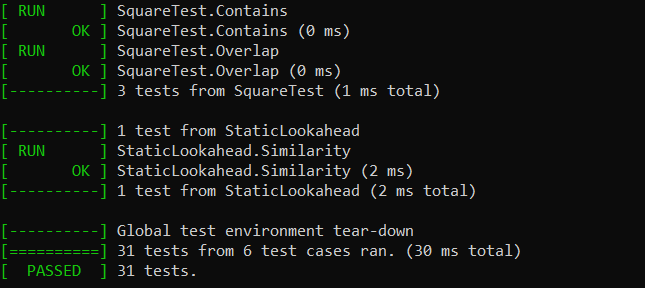
\includegraphics[width=0.6\textwidth]{sections/image/Unit.png}
    \caption{Unit Test Completion}
\end{figure}

\subsubsection{TSP File System}
\label{filesystem}

Tsp\_file(Section\ref{sec:TSP_File}) refers to the naming convention and type of data that is being stored. For the use-case of storing test results, the file needs to be stored in a dynamically sized list of tsp\_file entries for appending and reading the results. No standard exists, so the choice of file format is made by the developer. Text-based formats like JSON\cite{rfc8259} are human readable and scheme free. C++ does not have the modern compiler reflection feature\cite{reflectiveprogramming}, which would allow the compiler to modify its own behaviour based on its own code. This feature is used by most JSON libraries outside C++ to serialise and deserialise class structure automatically; for C++, the conversion has to be manually defined which could introduce errors if not adequately tested.

The files produced by the empirical testing are illegible for human use due to excessive data in an illogical format. Therefore, an application, TSP\_Reader, that can deserialise, analyse, and reproduce more legible data is beneficial. TSP\_Reader uses the TSP file system to process the file, uses data processing to transform the data into a more readable form, and then uses the libxlsxwriter library(Section\ref{cpplibrar}) to create an Excel file with tables and graphs. The data is processed based on problem size(Figure\ref{Excel1}) and algorithm(Figure\ref{Excel2}).

\begin{figure}[H]
    \centering
    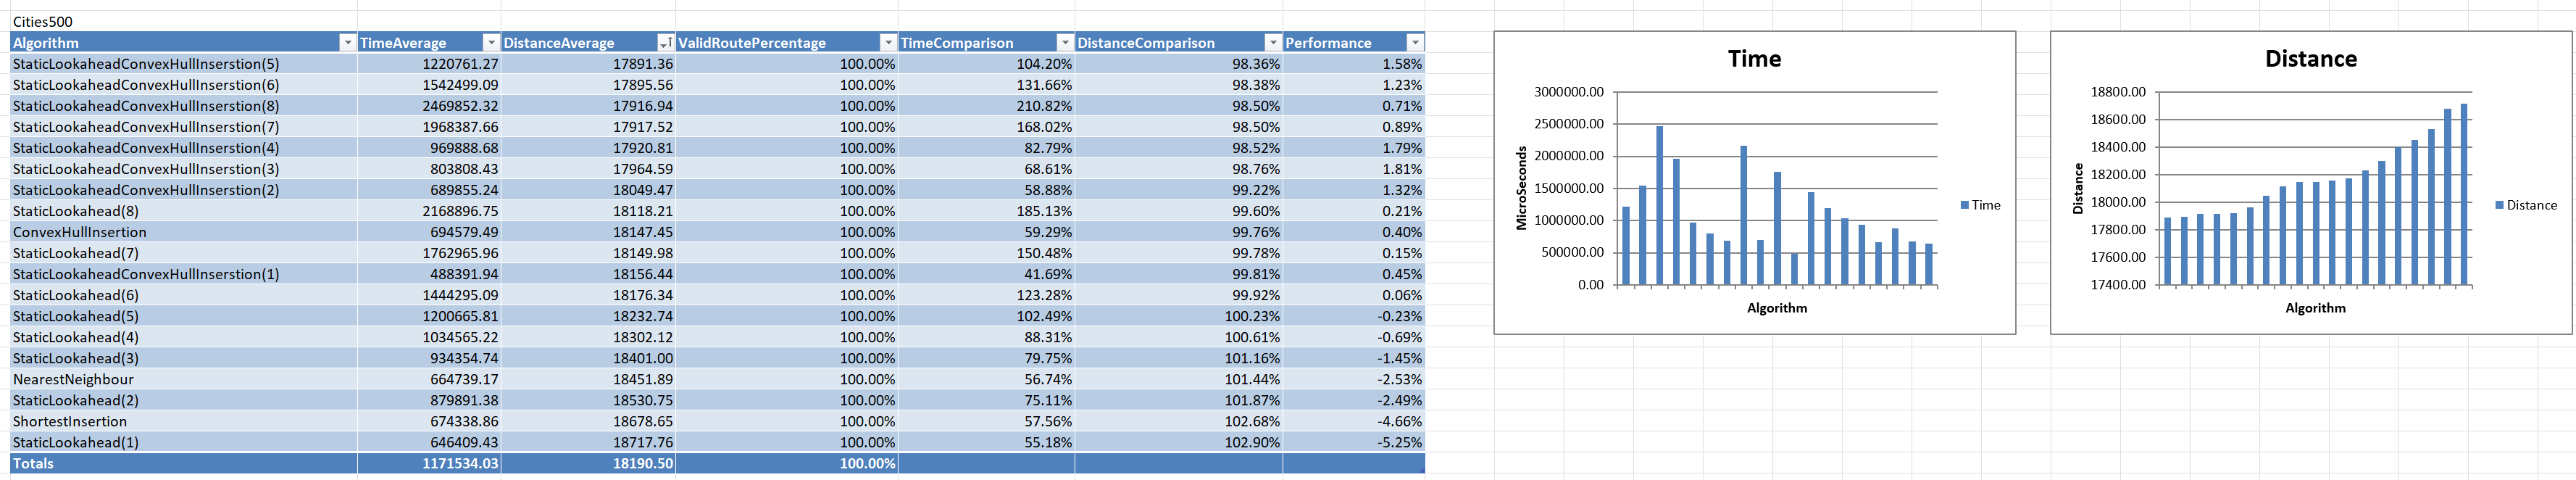
\includegraphics[width=\textwidth]{sections/image/excelfile.png}
    \caption{Excel File - Based On Size}
    \label{Excel1}
\end{figure}
\begin{figure}[H]
    \centering
    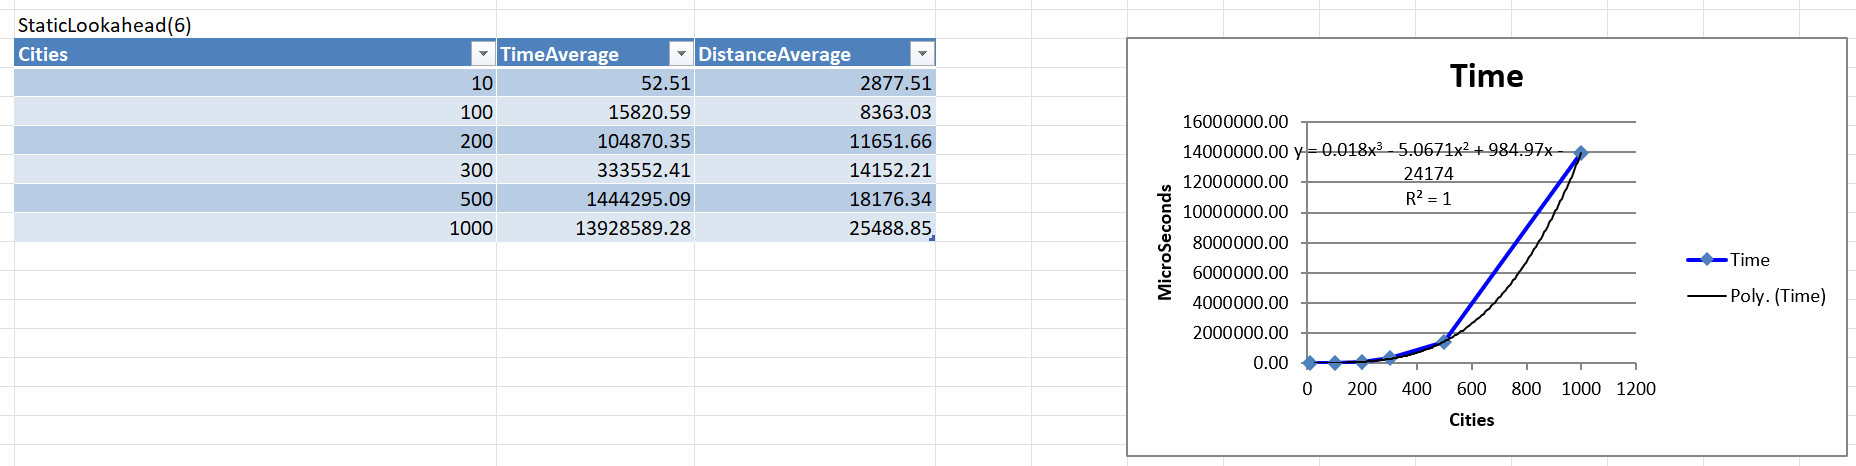
\includegraphics[width=\textwidth]{sections/image/ExcelFile2.png}
    \caption{Excel File - Based On Algorithm}
    \label{Excel2}
\end{figure}
